\documentclass[12pt]{article}
\usepackage{amsmath}
\usepackage{graphicx}
\usepackage{caption}
\usepackage{float}
\usepackage[utf8]{inputenc}
\usepackage{geometry}
\usepackage{svg}
\usepackage{listings}
\usepackage{xcolor}
\usepackage{longtable}
\usepackage{polski}
\geometry{a4paper, margin=1in}

\title{Zadanie 3 z Metod Probabilistycznych i Statystyki}
\author{Mikołaj Krupiński}
\date{Styczeń 2023}

\definecolor{codegreen}{rgb}{0,0.6,0}
\definecolor{codegray}{rgb}{0.5,0.5,0.5}
\definecolor{codepurple}{rgb}{0.58,0,0.82}
\definecolor{backcolour}{rgb}{0.95,0.95,0.92}

\lstdefinestyle{mystyle}{
  backgroundcolor=\color{backcolour},   commentstyle=\color{codegreen},
  keywordstyle=\color{magenta},
  numberstyle=\tiny\color{codegray},
  stringstyle=\color{codepurple},
  basicstyle=\ttfamily\footnotesize,
  breakatwhitespace=false,         
  breaklines=true,                 
  captionpos=b,                    
  keepspaces=true,                 
  numbers=left,                    
  numbersep=5pt,                  
  showspaces=false,                
  showstringspaces=false,
  showtabs=false,                  
  tabsize=2
}

\lstset{style=mystyle}

\begin{document}

\maketitle

\section{Zadanie 1}
Celem zadania jest poddanie testom NIST generatorów liczb losowych z różnych języków programowania, w celu oceny ich właściwości statystycznych.

\subsection*{Generator typu LCG}
Testom poddałem ciąg bitów długości 2 milionów wygenerowanych przez funkcję $rand()$ z języka C. Generator zainicjowałem aktualnym czasem UNIX'owym komputera.

\begin{figure}[H]
    \centering
    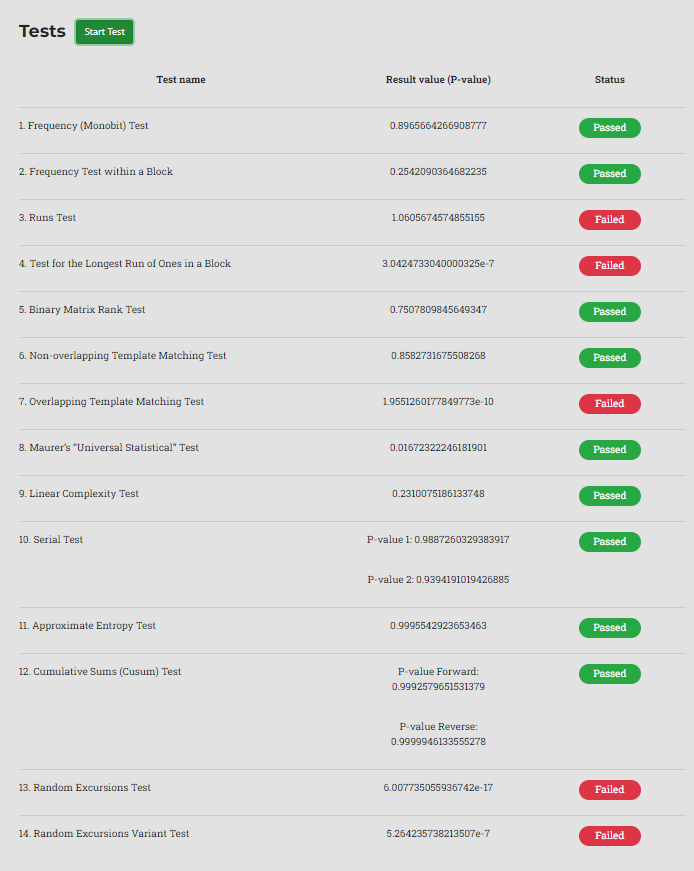
\includegraphics[width=10cm, clip]{images/z1a.png}
\end{figure}

Jak widać na zrzucie ekranu generator LCG nie przeszedł przez 5 z 14 testów, więc nie może być używany do eksperymentów probabilistycznych, ponieważ wyniki mogą być przekłamane.

\subsection*{Generator typu Mersenne Twister}
Testom ponownie poddałem ciąg bitów długości 2 milionów, jednak tym razem użyłem implementacji generatora $Mersenne$ $Twister$ w języku C++.

\begin{figure}[H]
    \centering
    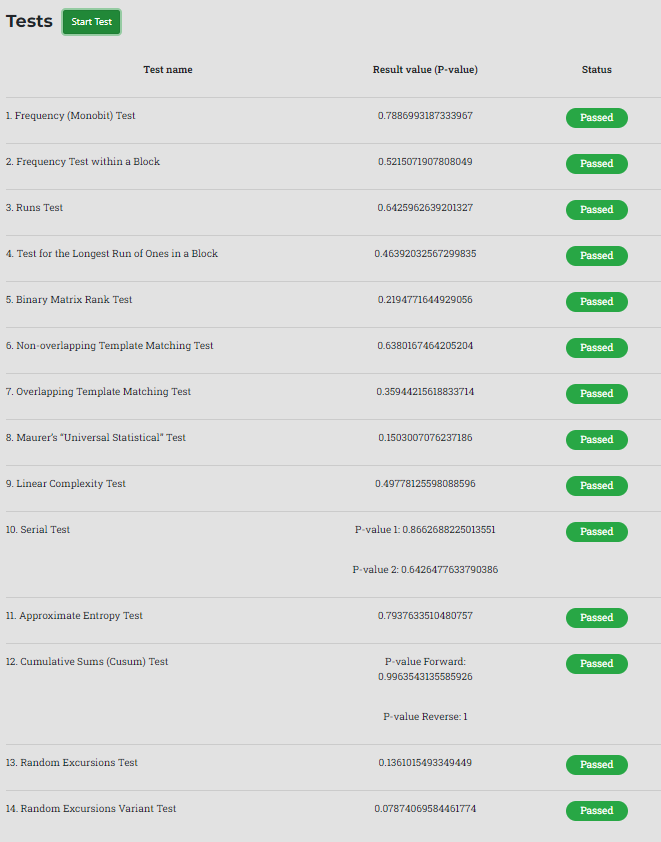
\includegraphics[width=10cm, clip]{images/z1b.png}
\end{figure}

Wygenerowany ciąg bitów przeszedł wszystkie testy, co oznacza że ma dobre właściwości statystyczne, jest nieodróżnialny od rzutu monetą. Można więc go używać do eksperymentów probabilistycznych.

\subsection*{Funkcja hashująca SHA-1}
Testom poddałem wynik działania funkcji SHA-1() dla mojego nazwiska.

\begin{figure}[H]
    \centering
    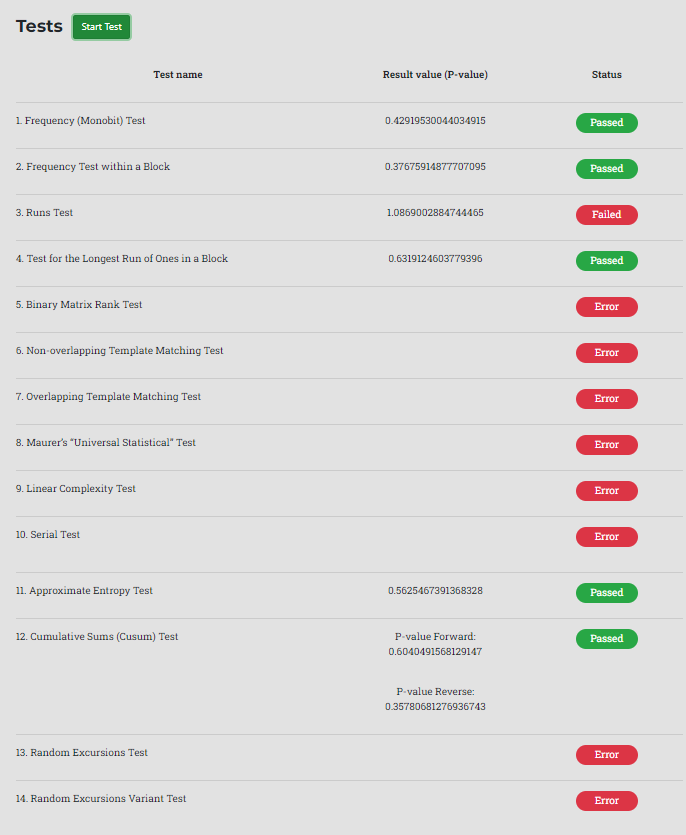
\includegraphics[width=10cm, clip]{images/z1c.png}
\end{figure}

Output funkcji hashującej przeszedł pomyślnie wszystkie testy, w których zostały spełnione wymagania, tzn. odpowiednia ilość bitów. Testy które zakończyły się błędem wymagają dużo więcej bitów (nawet milion), aby ich wyniki były wiarygodne.

\section{Zadanie 2}
Celem zadania jest wyznaczenie numerycznie dystrybuanty zmiennej losowej $S_N = \sum_{n=1}^{N}X_n$, gdzie poszczególne $X_i$ są niezależne i przyjmują wartości -1 oraz 1 z prawdopodobieństwem 0.5. W tym celu napisałem skrypt w $Matlab'ie$, który dla danego $N$ generuje 10000 losowych wartości zmiennej $S_N$.

\begin{lstlisting}[language=Matlab, caption=custom\_dist.m]
S = zeros(10000, 1);
N = 100;
    
for i = 1:10000
    X = randi([0 1], 1, N);
    X(X == 0) = -1;
    S(i) = sum(X);
end

cdfplot(S);
hold on;
pd = makedist('Normal', 'mu', 0, 'sigma', sqrt(N));
x = -40:.1:40;
p = cdf(pd, x);
plot(x, p);
\end{lstlisting}

Otrzymane wyniki dla $N \in \{5,10,15,20,25,30,100\}$ przedstawiłem na wspólnych wykresach z rozkładem normalnym o odpowiednich parametrach, tzn. średniej 0 i odchyleniu standardowym $\sqrt{N}$. Są to oczywiście parametry rozkładu zmiennej $S_N$. Te wynikają z tego, że $E(X_i)=0$ oraz $Var(X_i)=1$ oraz z addydtywności wartości oczekiwanej i wariancji i zależności wariancji od odchylenia standardowego. \par
Na każdym z poniższych wykresów niebieskim kolorem narysowana jest dyskretna dystrybuanta zmiennej $S_N$, natomiast na czerwono dystrybuanta rozkładu normlanego.

\begin{figure}[H]
    \centering
    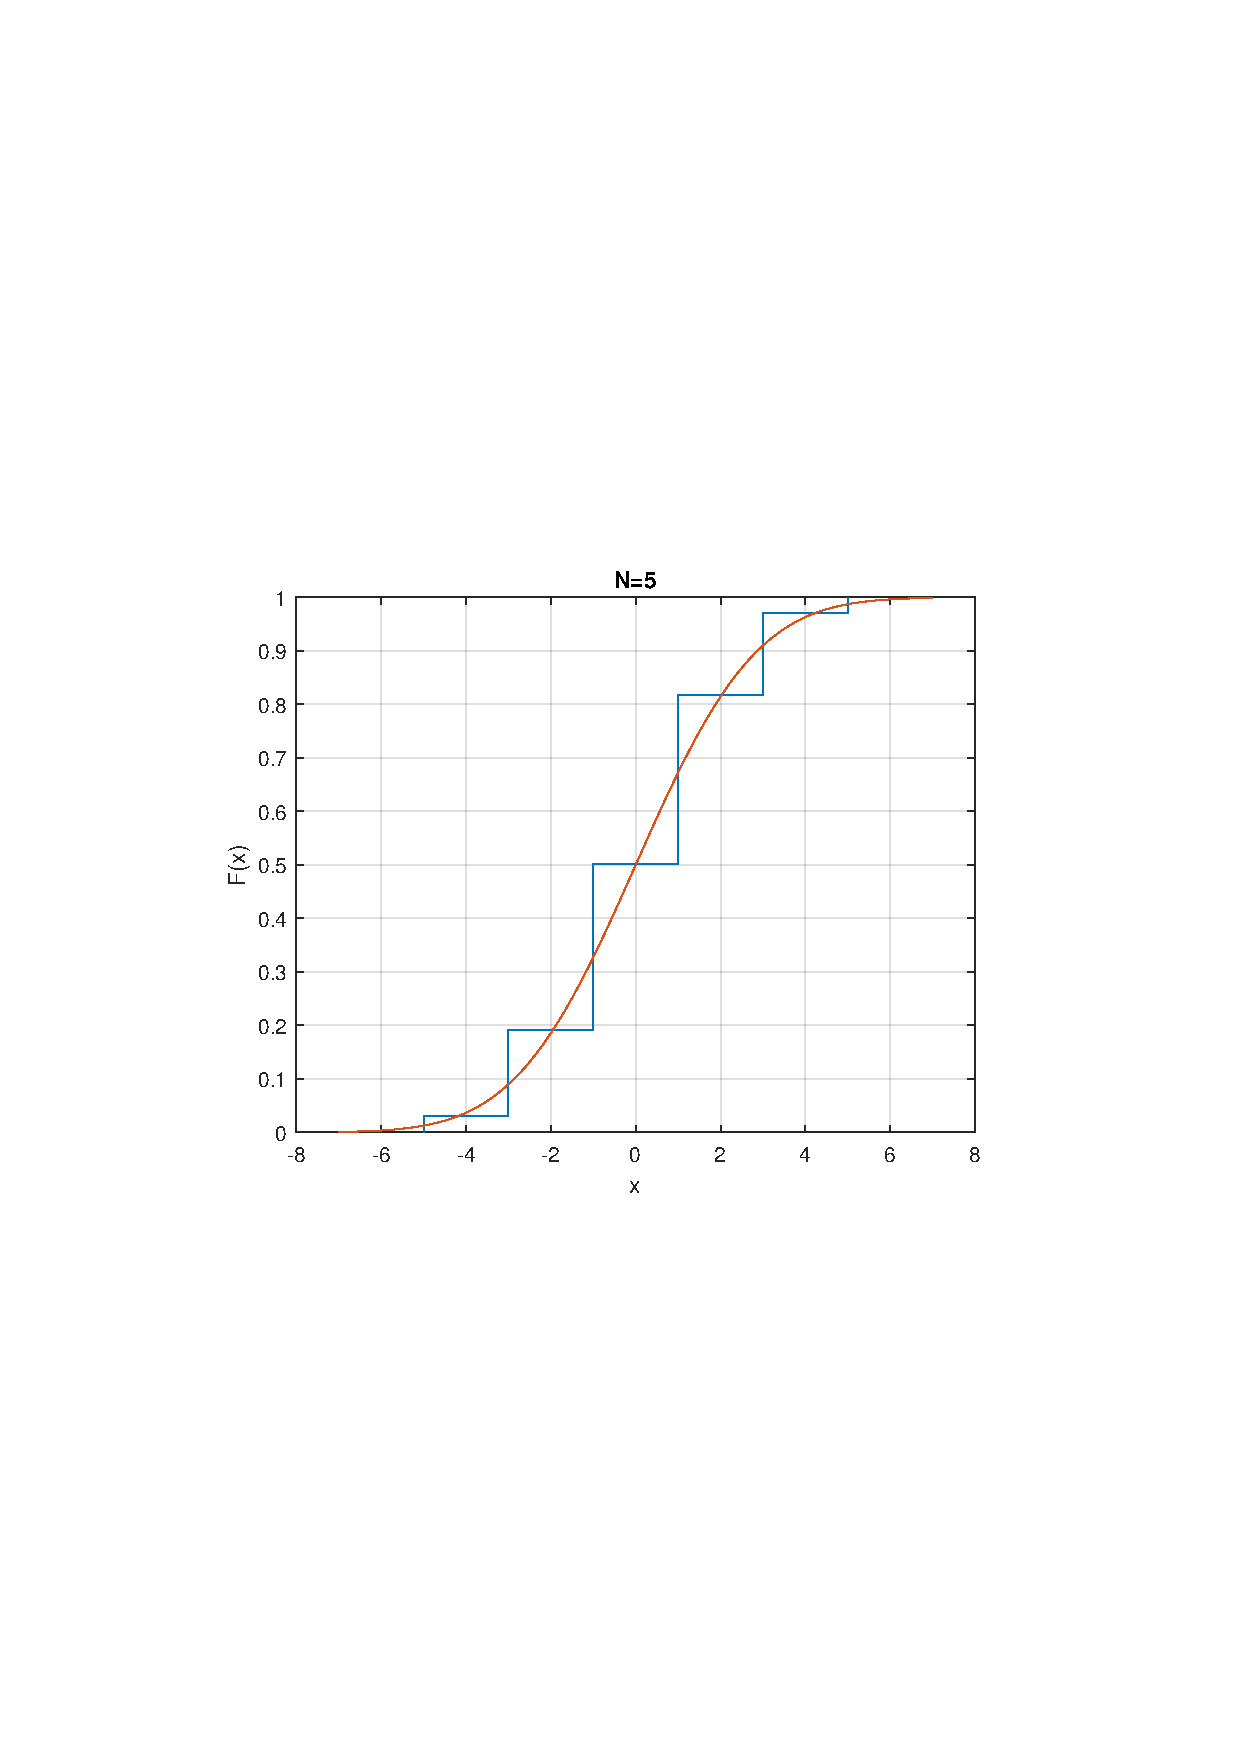
\includegraphics[width=15cm, trim = 0 9cm 0 9cm, clip]{images/z25.pdf}
\end{figure}
\begin{figure}[H]
    \centering
    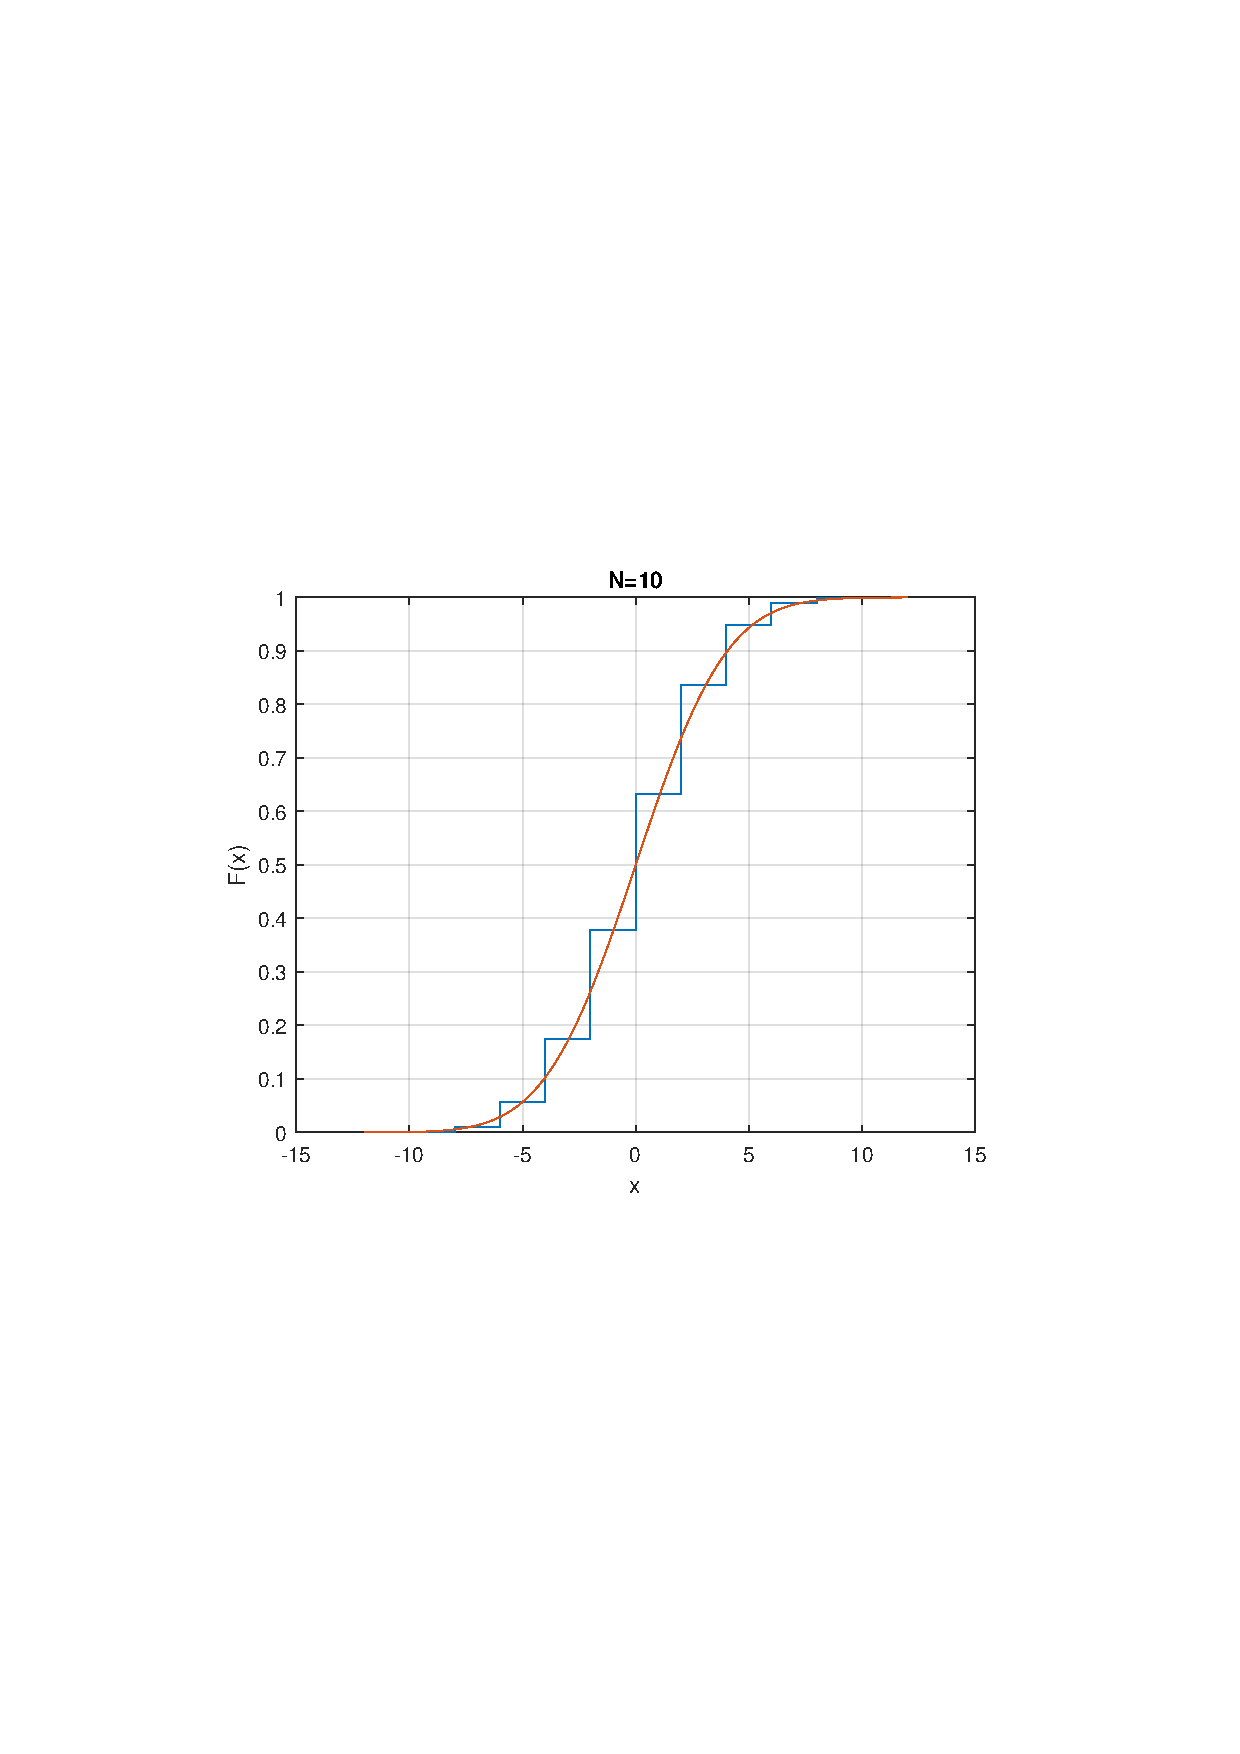
\includegraphics[width=15cm, trim = 0 9cm 0 9cm, clip]{images/z210.pdf}
\end{figure}
\begin{figure}[H]
    \centering
    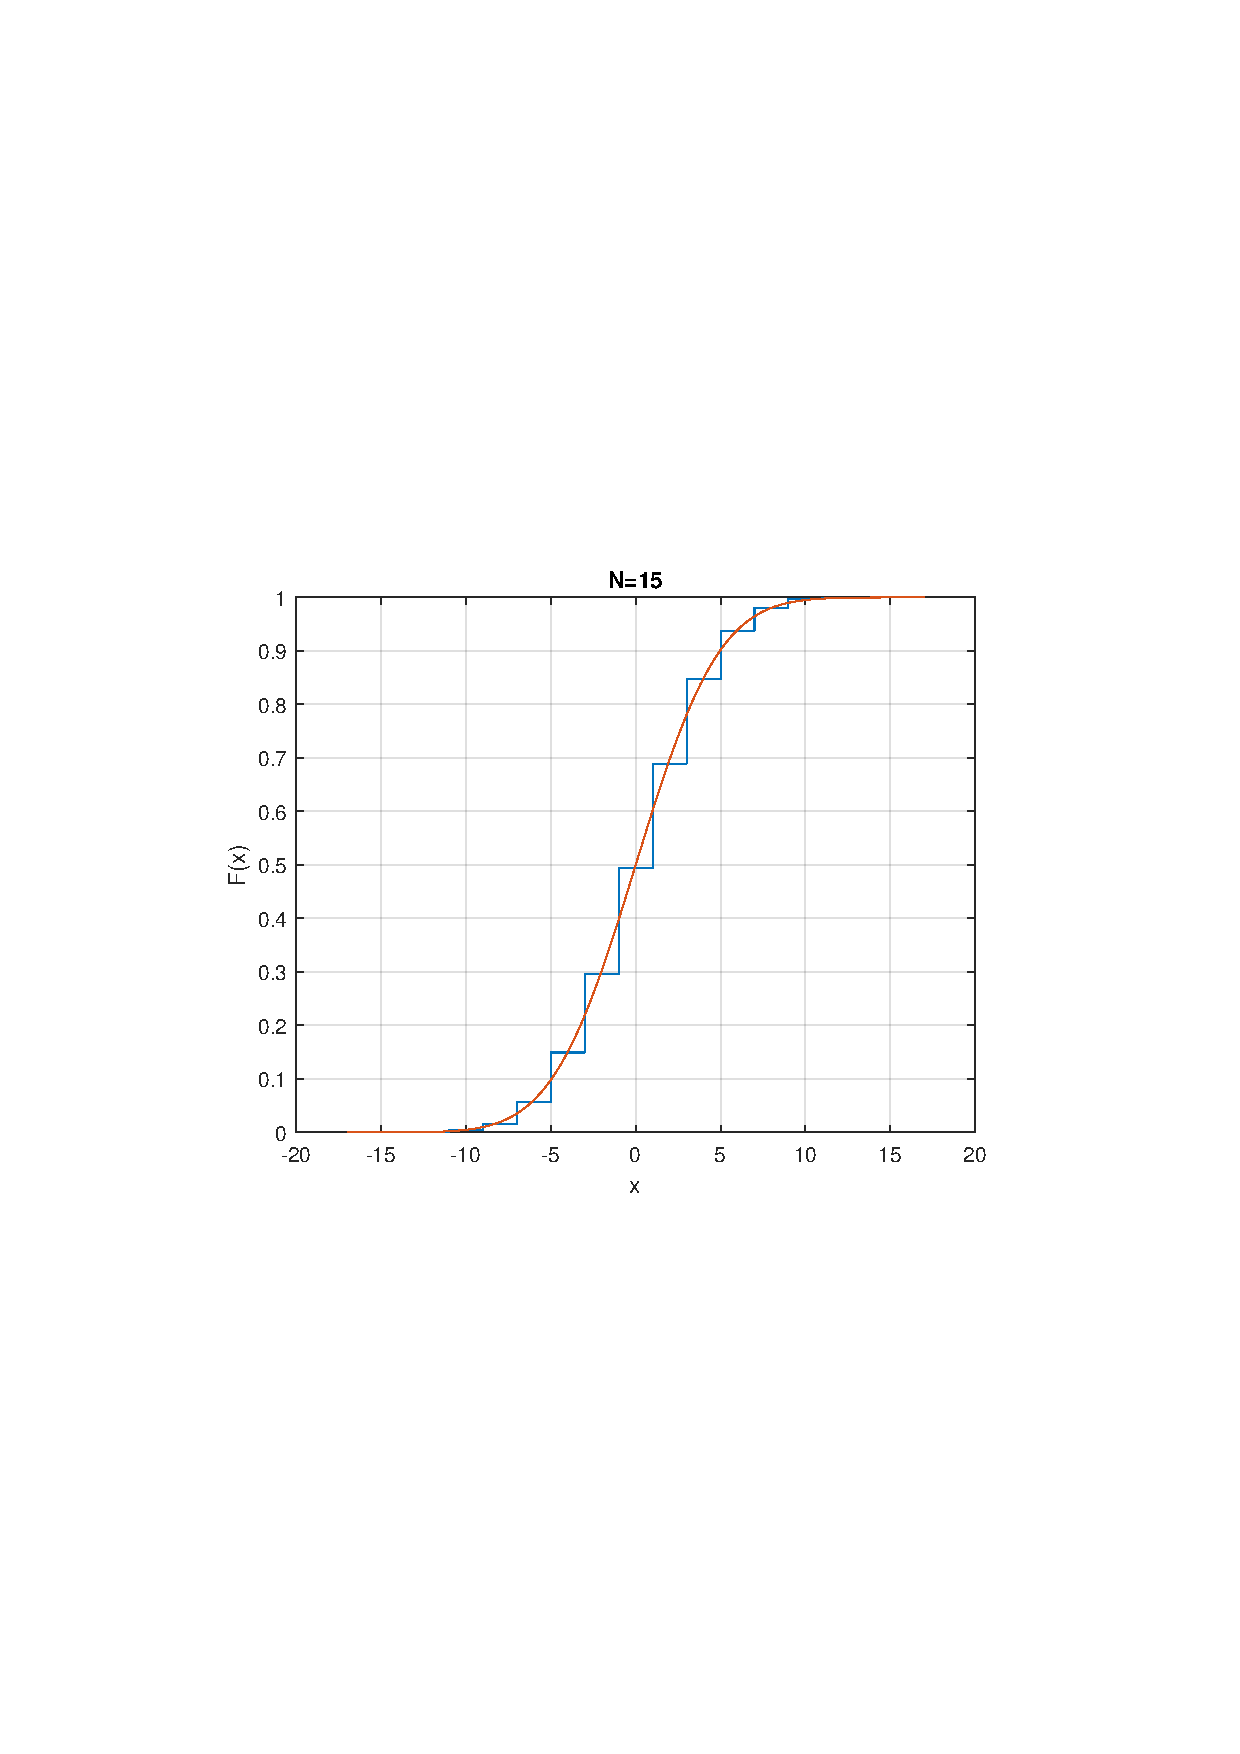
\includegraphics[width=15cm, trim = 0 9cm 0 9cm, clip]{images/z215.pdf}
\end{figure}
\begin{figure}[H]
    \centering
    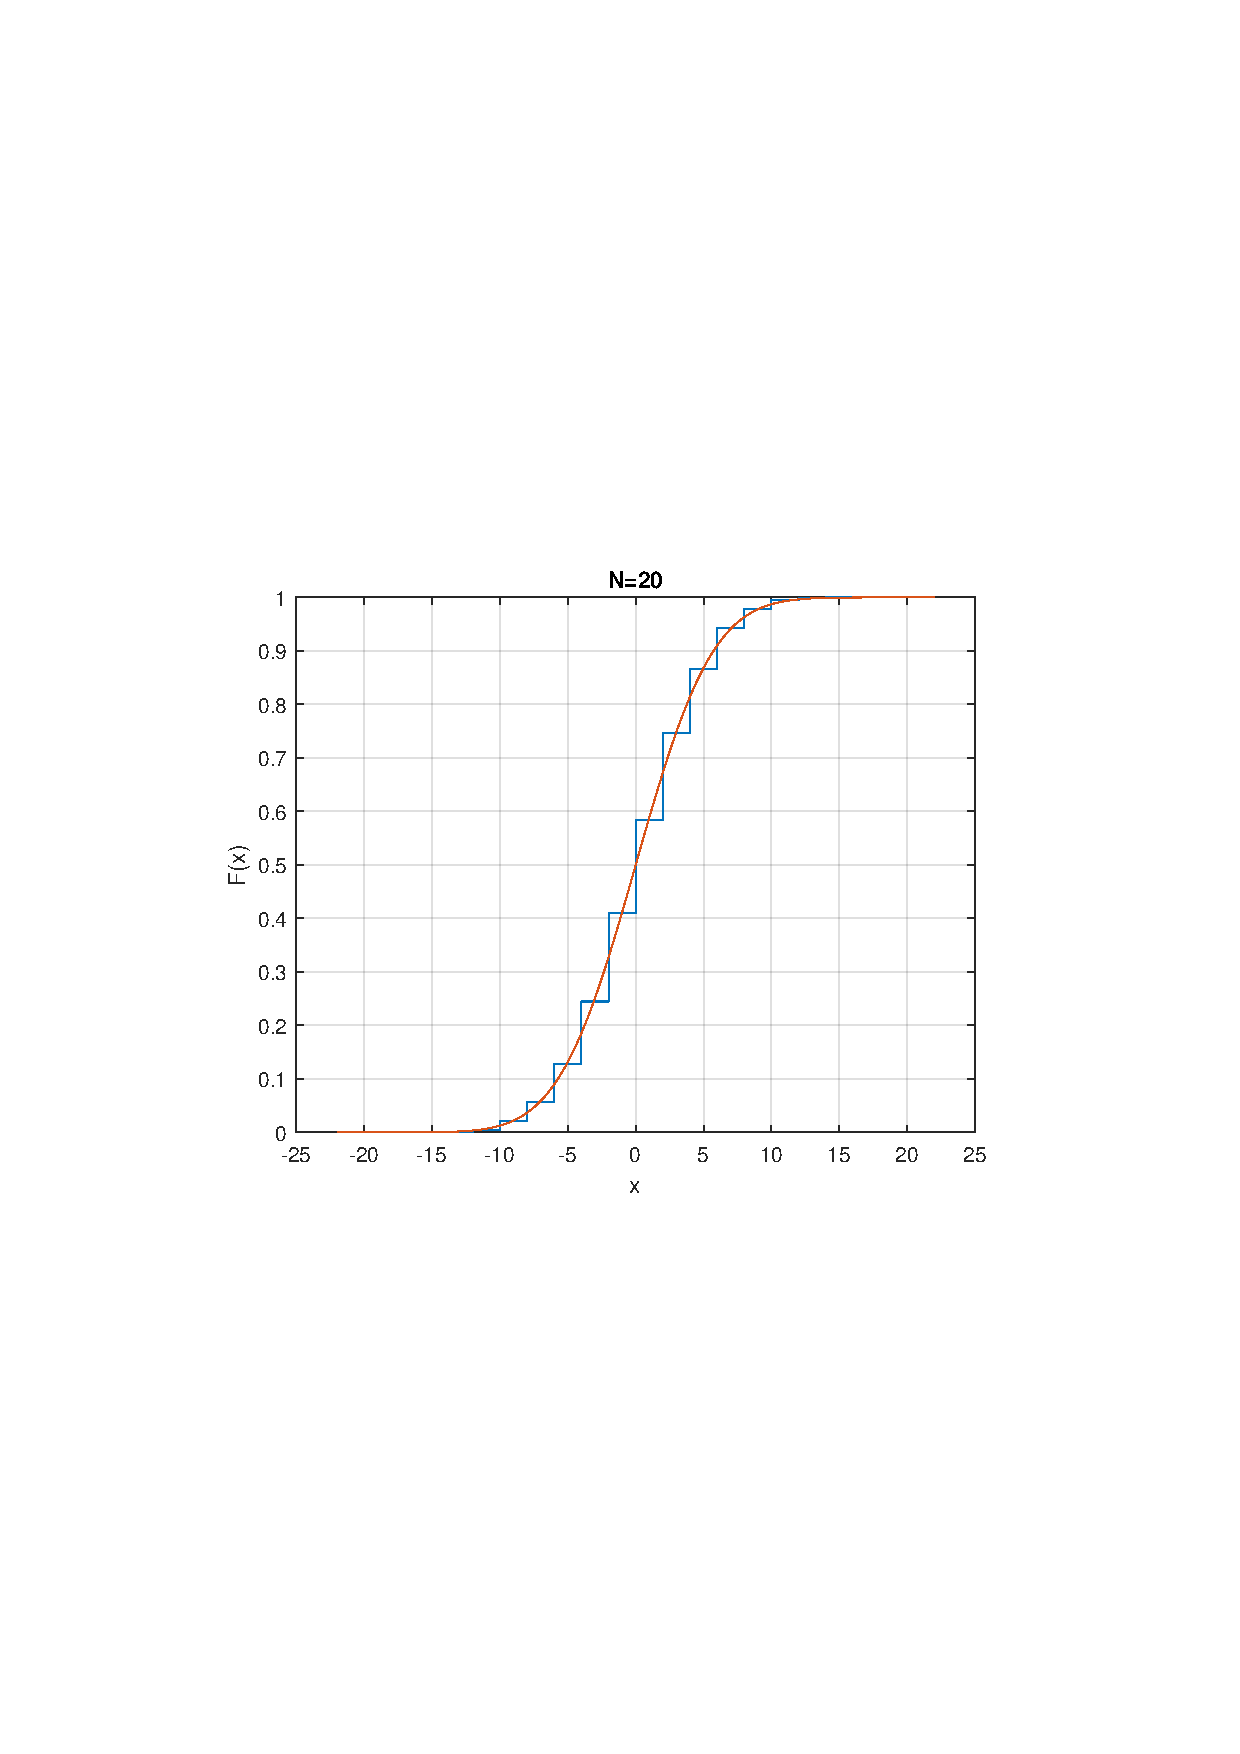
\includegraphics[width=15cm, trim = 0 9cm 0 9cm, clip]{images/z220.pdf}
\end{figure}
\begin{figure}[H]
    \centering
    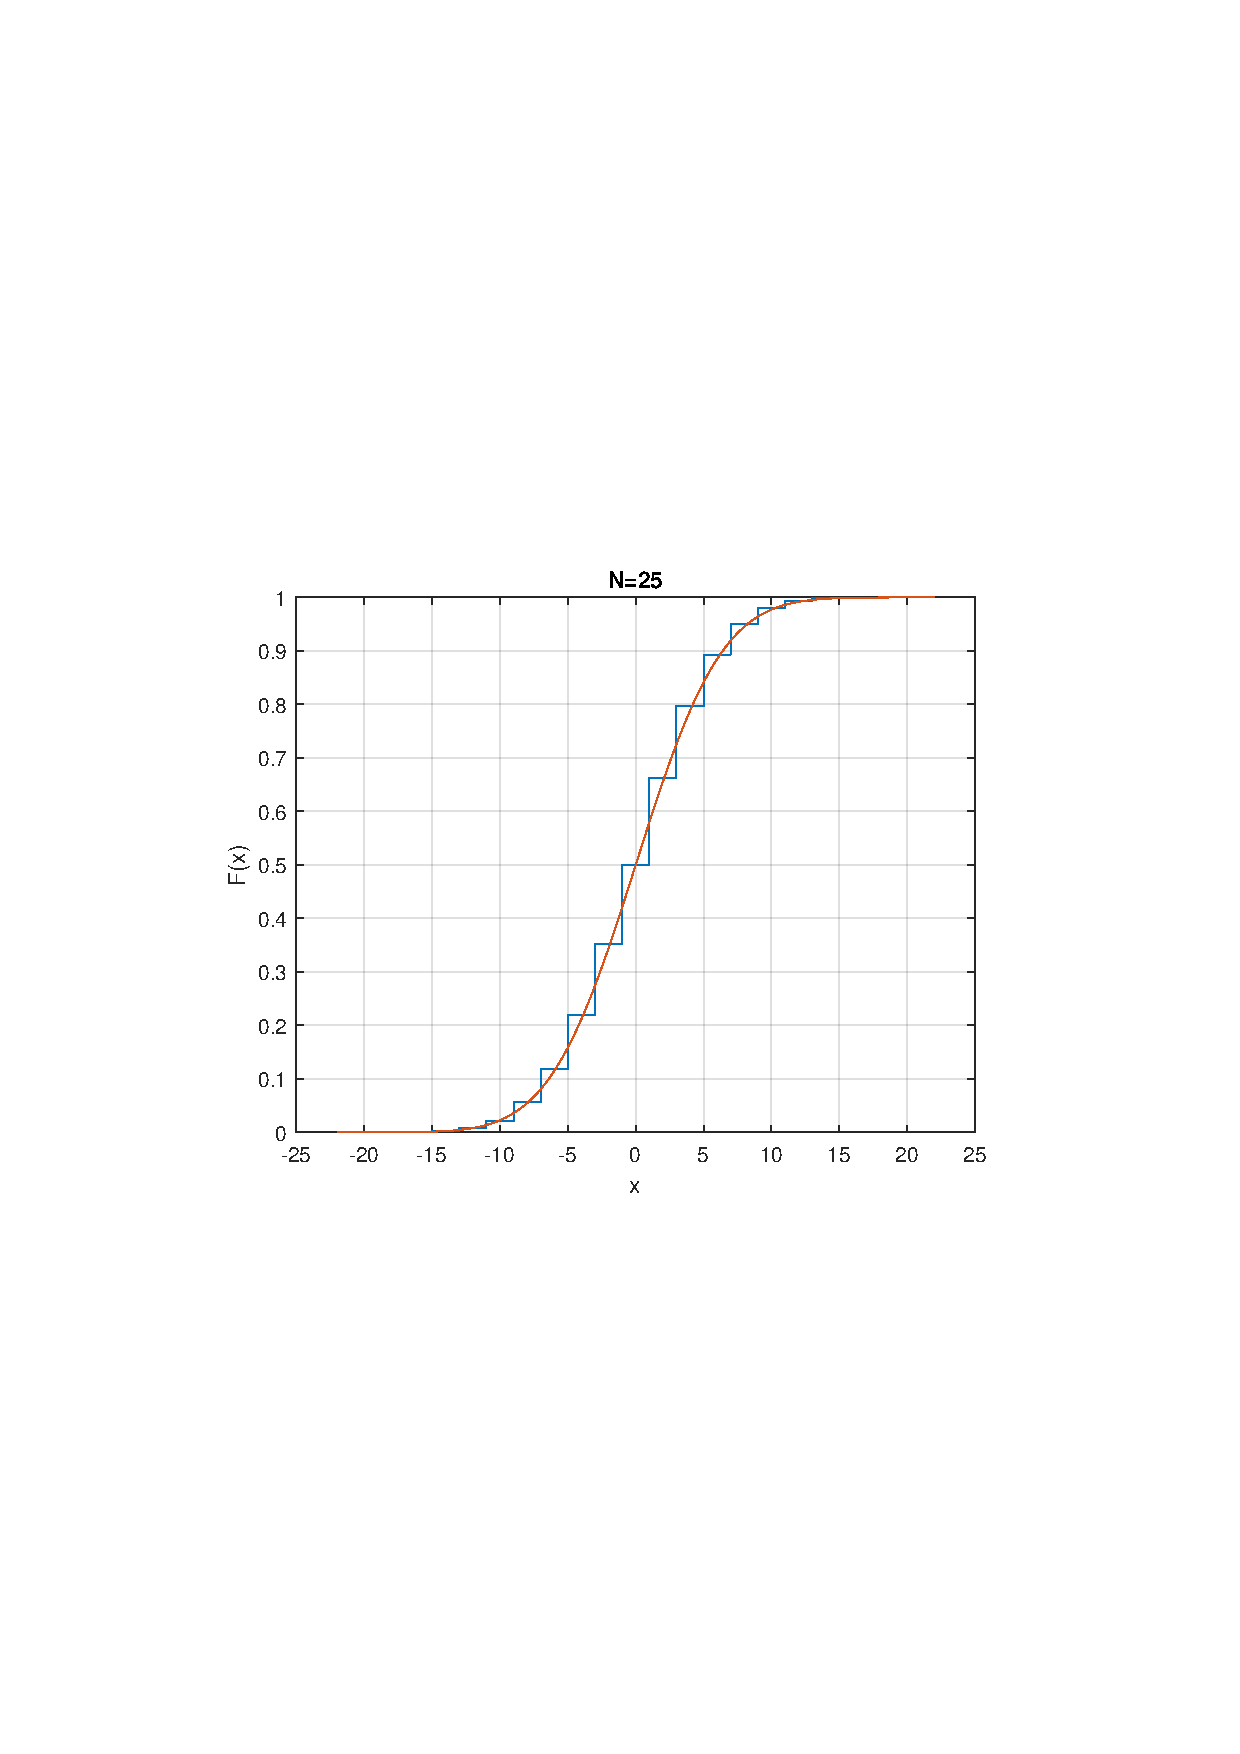
\includegraphics[width=15cm, trim = 0 9cm 0 9cm, clip]{images/z225.pdf}
\end{figure}
\begin{figure}[H]
    \centering
    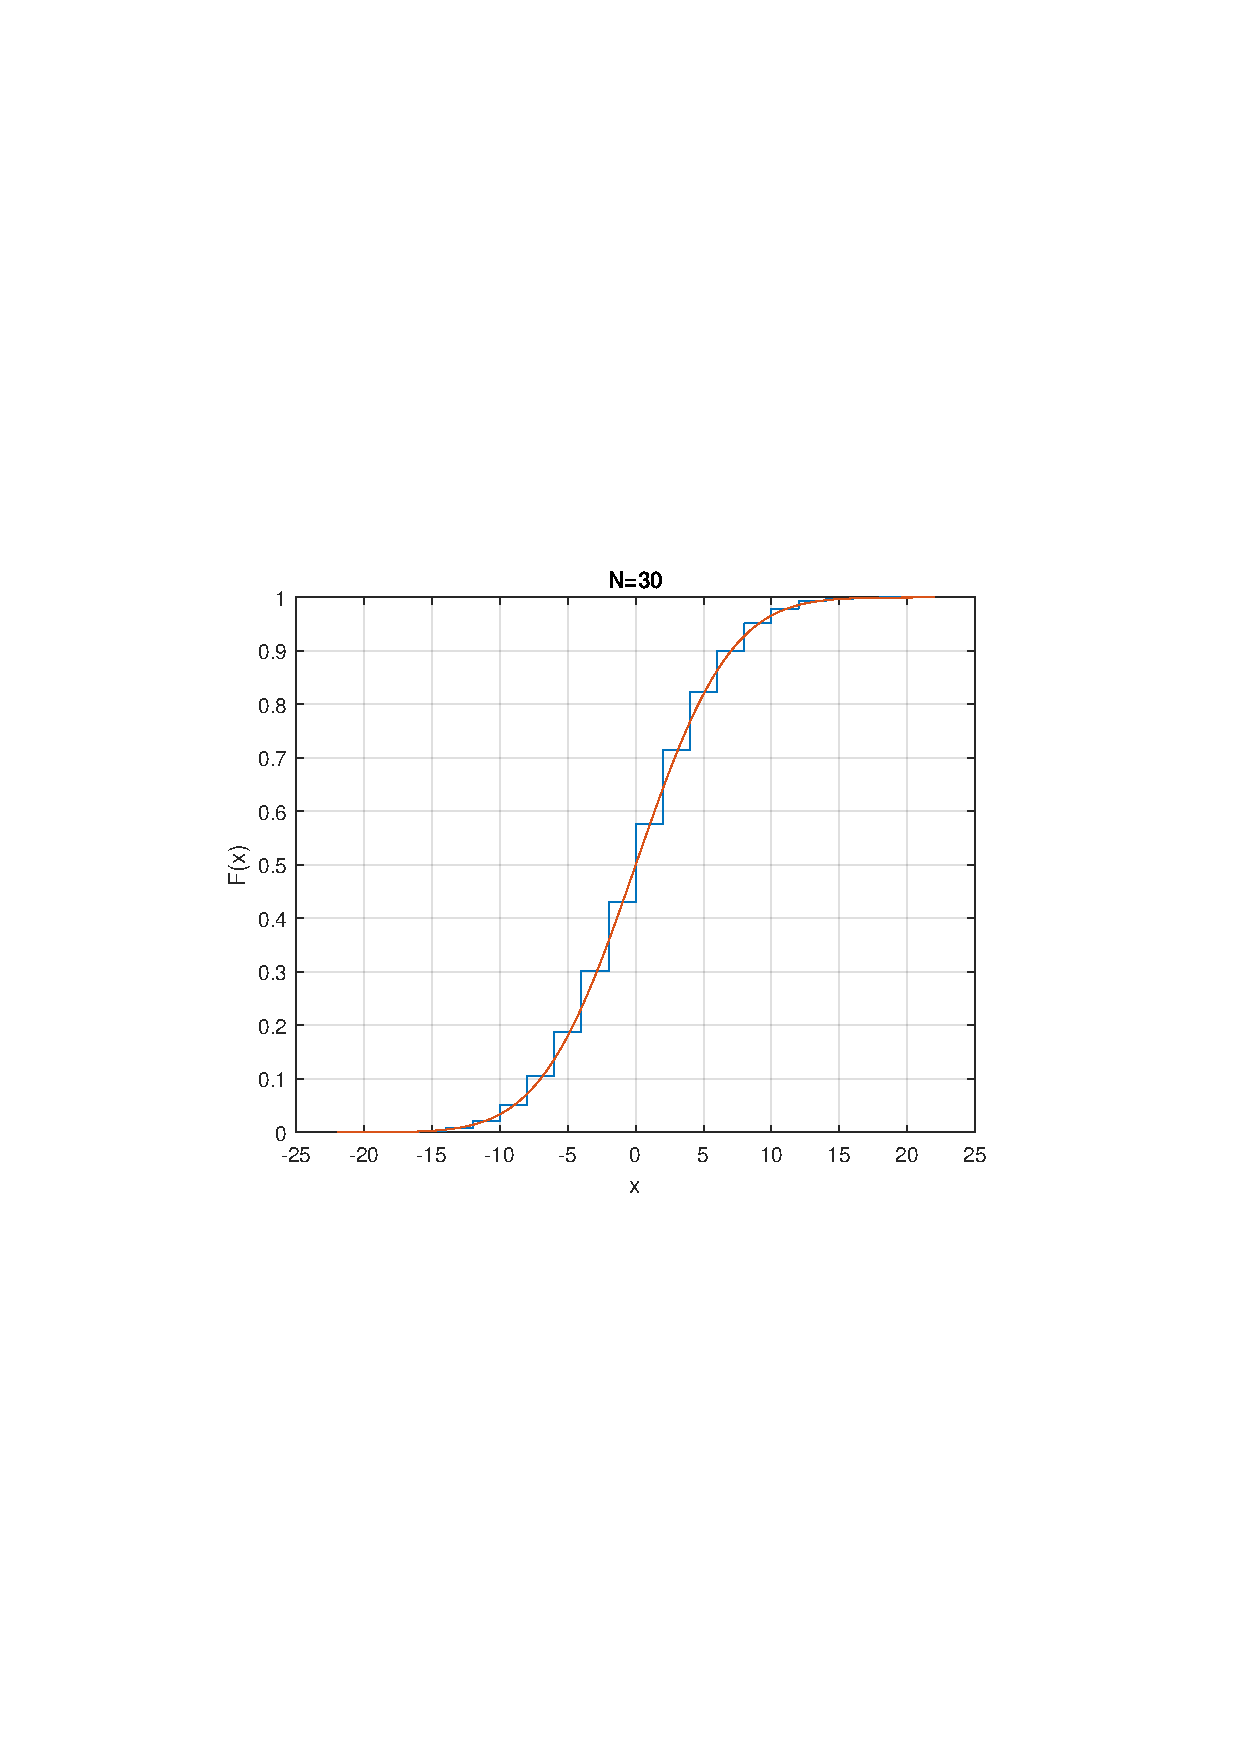
\includegraphics[width=15cm, trim = 0 9cm 0 9cm, clip]{images/z230.pdf}
\end{figure}
\begin{figure}[H]
    \centering
    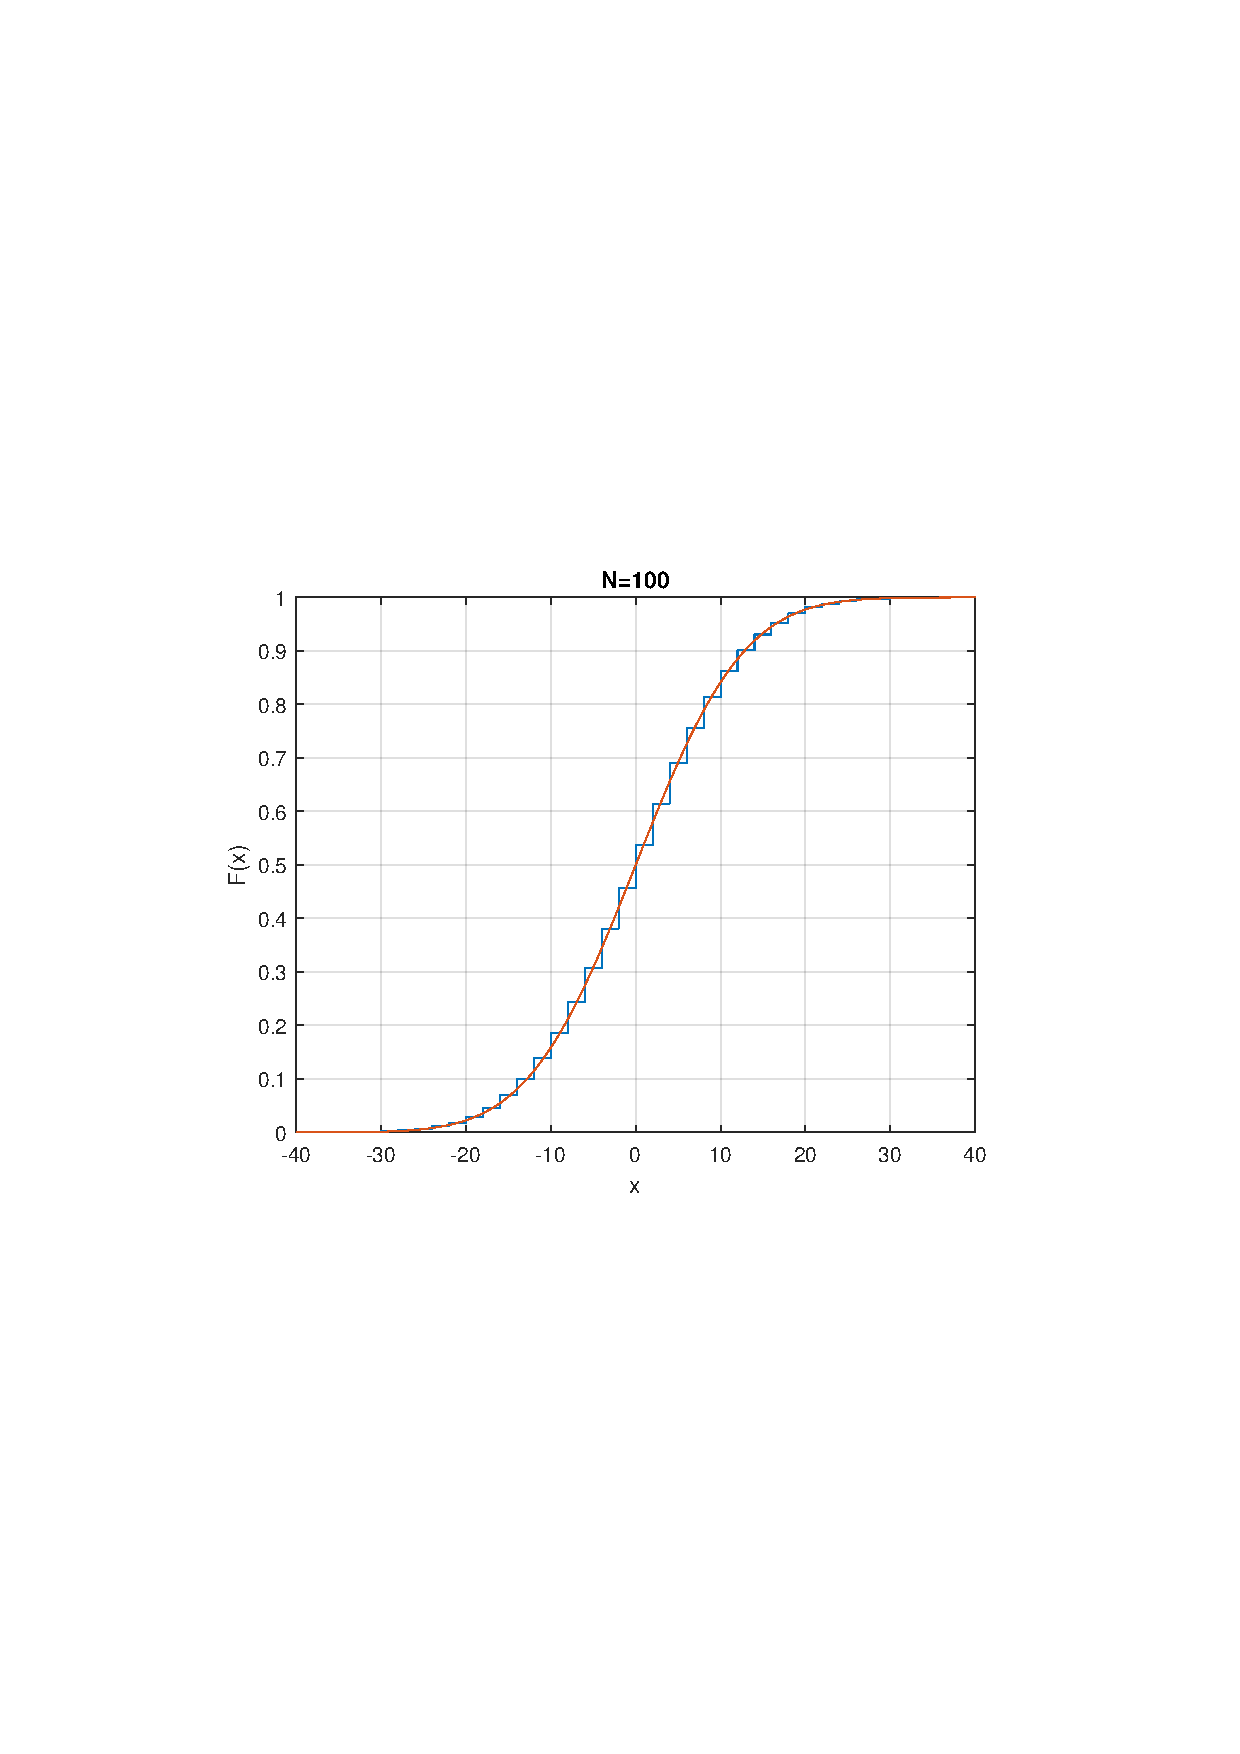
\includegraphics[width=15cm, trim = 0 9cm 0 9cm, clip]{images/z2100.pdf}
\end{figure}

Na każdym z wykresów widać mocną zależność między sumą zmiennych $X_i$ a rozkładem normalnym. Zaskakujące jest, że już dla $N=5$ wykresy się praktycznie pokrywają z dokładnością do jedności. Dla większych $N$ przybliżenie sumy zmiennych losowych o tej samej wartości oczekiwanej i wariancji rozkładem normalnym jest bardzo dokładne. Widać, że wzrost dokładności estymacji jest ściśle związany z ilością sumowanych zmiennych.

\section{Zadanie 3}
Celem tego zadania jest eksperymentalne wyznaczenie rozkładu czasu spędzonego nad osią $OX$ (oznaczenie: $P_N$) przy błądzeniu losowym, tzn. w każdym kroku ruch wykonywany jest do góry lub w dół z jednakowym prawdopodobieństwem. \par
W celu wyznaczenia rozkładu zmiennej $P_N$ napisałem program w języku $C++$, w którym symuluję błądzenie losowe dla $N=100,1000,10000$ za każdym razem powtarzając eksperyment $k=5000$ razy. Wyliczone wartości zapisuję do plików (do późniejszej analizy).

\begin{lstlisting}[language=C++, caption=generate\_data.cpp]
#include <iostream>
#include <random>
#include <ctime>
#include <fstream>
    
int main()
{
    std::mt19937 urbg {(unsigned int)time(NULL)};  
    std::uniform_int_distribution<int> distr1 {0, 1};
    
    std::ofstream f2("data2.txt");
    std::ofstream f3("data3.txt");
    std::ofstream f4("data4.txt");
        
    for (int n = 100; n <= 10000; n *= 10)
    {
        for (int k = 0; k < 5000; k++)
        {
            int position = 0;
            int L = 0;
    
            for (int i = 0; i < n; i++)
            {
                int step = distr1(urbg) == 0 ? -1 : 1;
                position += step;
                    
                if (position > 0 || (position == 0 && step == -1))
                    L++;
            }
    
            double P = L * 1.0 / n;
    
            if (n == 100)
                f2 << P << (k != 4999 ? "," : "\n");
            else if (n == 1000)
                f3 << P << (k != 4999 ? "," : "\n");
            else
                f4 << P << (k != 4999 ? "," : "\n");;
    
        }
    }
        
    f2.close();
    f3.close();
    f4.close();
    
    return 0;
}
\end{lstlisting}

Na wykresach brązowe słupki oznaczają wyznaczoną numerycznie gęstość rozkładu $P_N$, natomiast niebieska linia to gęstość rozkładu arcsin. \par

\subsection*{Wykres dla $N=100$}
\begin{figure}[H]
    \centering
    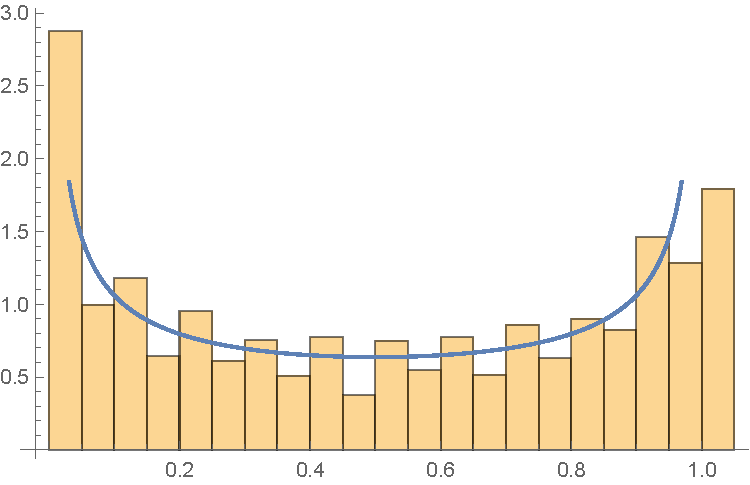
\includegraphics[width=15cm, clip]{images/z3100.pdf}
\end{figure}
\subsection*{Wykres dla $N=1000$}
\begin{figure}[H]
    \centering
    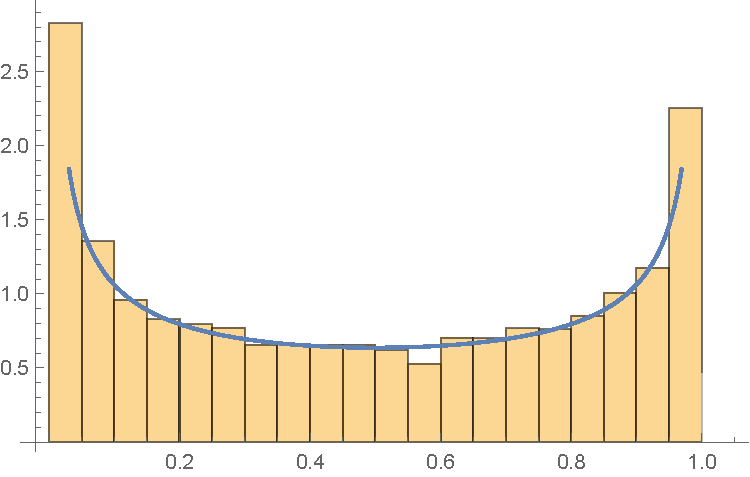
\includegraphics[width=15cm, clip]{images/zad31000.pdf}
\end{figure}
\subsection*{Wykres dla $N=10000$}
\begin{figure}[H]
    \centering
    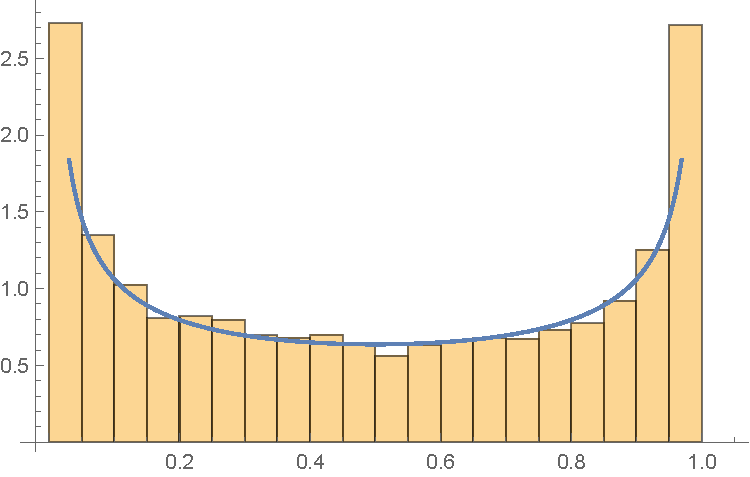
\includegraphics[width=15cm, clip]{images/z310000.pdf}
\end{figure}

Jak widać na wykresach zmienna losowa $P_N$ ma rozkład bardzo zbliżony do rozkładu arcsin. Dla $N=100$ nie jest to aż tak wyrażna zależność, jednak wraz ze wzrostem liczby kroków w błądzeniu $P_N$ coraz bardziej zbliża się do rozkładu arcsin. Dla $N=10000$ wykresy się praktycznie pokrywają. \par
Zaskakującym dla mnie wnioskiem jest, że najbardziej prawdopodbne jest spędzenie bardzo mało albo bardzo dużo czasu nad osią $OX$, a nie jak intuicyjnie by się wydawało połowy czasu.

\end{document}